%-----------------------------------------------------------------------------------------------------------------
%% Section 1
\chapter{Question 1: Heat Exchanger Circuit}
\label{chap:q1}

The constant parameters given for the first question are summarized below in Table~\ref{tab:q1param} as per \cite{assign}.

\begin{table}[H]
  \centering
  \caption{Constant parameters for Question 1.}
    \begin{tabular}{cccc}
	\toprule    
    \textbf{Description} & \textbf{Symbol} & \textbf{Value } & \textbf{Unit} \\
    \midrule
    Tubing diameter 		& $D$     & 1.25  & in \\
    Specific gravity 		& $SG$    & 0.875  & - \\
    Kinematic viscosity 	& $\nu$    & 110   & cS \\
    Length of tube 			& $L$     & 55    & ft \\
    \bottomrule
    \end{tabular}
  \label{tab:q1param}
\end{table}

The foregoing subsections will use these values. Also note that all equations presented in this report are from \cite{formula}, unless stated otherwise. Furthermore, all numerical results calculated with \cite{excel}.

\section{Part A}
\label{sect:1a}

First, it is required to calculate the maximum velocity. The Reynolds number formula may be rearranged as per \ref{eq:re} to yield $v_{max}$.

\begin{equation}
	\label{eq:re}
	Re = \frac{v_{max}D}{\nu} \Rightarrow v_{max} = \frac{1}{7740} \frac{\nu Re}{D}
\end{equation}

Note, a factor of 1/7740 is added to convert [cS/in] to [ft/s]. Since it is stated that the flow is kept at the upper limit of the laminar flow range \cite{assign}, the Reynolds number is set to be $Re=2000$ as per \cite{fluids}.\\

From this, the maximum volumetric flow rate $Q_{max}$ is calculated with \ref{eq:flowq}.

\begin{equation}
	\label{eq:flowq}
	Q_{max} =  \frac{449}{144} v_{max} A	
\end{equation} 

Where the piping area is $ A = \frac{1}{4}\pi D^2 \Unit{[in^2]}$. The above equation yields [$\Unit{\frac{ft^3}{s}}$] hence to get [gpm], the equation is multiplied by 449/144. Calculated maximum velocity, area and flow rate are summarized below in Table~\ref{tab:q1ans1}.

\begin{table}[H]
  \centering
  \caption{Calculated velocity, area and volumetric flow rate.}
    \begin{tabular}{cccc}
    \toprule
    \textbf{Description} & \textbf{Symbol} & \textbf{Value } & \textbf{Unit} \\
    \midrule
    Maximum velocity	& $v_{max}$	& 22.739	& ft/s \\
    Pipe area 			& $A$     	& 1.227 	& $\Unit{in^2}$ \\
    Maximum flow 		& $Q_{max}$	& 87.009 	& gpm \\
    \bottomrule
    \end{tabular}
  \label{tab:q1ans1}
\end{table}

Next, it is required to calculate the total head loss $h_L$ throughout the length $L$ of pipe to get the pressure drop $\Delta p$.

\begin{equation}
	\label{eq:q1headloss}	
	h_L = \left( \sum_{i=1}^{n} K_i \right) \frac{v^2}{2g} 
\end{equation}
 
In Equation\ref{eq:q1headloss}, $\Sigma K_i$ is the sum of all hydraulic circuit loss factors. This also includes the overall pipe's loss factor $K_{PL}$ defined as \ref{eq:q1kpipeloss}.

\begin{equation}
	\label{eq:q1kpipeloss}	
	K_{PL} = f \frac{L}{D} = 12 \frac{SL}{Re D}
\end{equation}

Where $S,L$ are the pipe's shape factor and length, respectively (see Table~\ref{tab:q1param}). A factor of 12 is added to convert the diameter from [in] to [ft] (recall $f=S/Re$ for laminar flow \cite{fluids}).\\

Each component in the heat exchanger's circuit will have their own loss factor. The following  shows the value for each of the circuit's factors $K_i$ (see Table~\ref{tab:kfact}). These figures were determined by interpolating values from Table~6.5 of \cite{fluids}. Note that the control valve factor $K_V$ and quantities are taken from \cite{assign}.

\begin{table}[H]
  \centering
  \caption{$K$ factors for all circuit components.}
    \begin{tabular}{cccc}
    \toprule
    \textbf{Loss Factor} & \textbf{Symbol} & \textbf{Value } & \textbf{Qty.} \\
    \midrule
    Control valve & $K_V$ & 0.920 & 1 \\
    Tee   & $K_T$ & 1.700 & 1 \\
    Elbow, 90 degrees & $K_E$ & 1.363 & 3 \\
    Check valve, open & $K_{CV}$ & 2.700 & 1 \\
    Globe valve, open & $K_{GV}$ & 7.875 & 2 \\
    Pipe loss & $K_{PL}$ & 16.896 & 1 \\
    Sum product  & $\Sigma K_i$   & 42.054 & - \\
    \bottomrule
    \end{tabular}
  \label{tab:kfact}
\end{table}

Next, the total head and pressures losses are computed with Equations~\ref{eq:q1headloss} and \ref{eq:q1ploss}, respectively. 

\begin{equation}
	\label{eq:q1ploss}	
	\Delta p = \frac{1}{144}\gamma_f h_L + \Delta p_F + \Delta p_{HE} 
\end{equation}

Where $\gamma_f = SG\  \gamma_{H20} \ [\Unit{lb/ft^3}]$ is the specific weight of the fluid. Values for  $SG,\ \gamma_{H20}$ taken from Table~\ref{tab:q1param} and \cite{fluids}, respectively. The first term of Equation~\ref{eq:q1ploss} is multiplied by 1/144 to convert from [$\Unit{lb/ft^2}$] to [$\Unit{lb/in^2}$] or [psi]. Pressure losses caused by the filter $\Delta p_F$ and heat exchanger $\Delta p_{HE}$ are given in \cite{assign} as 5.5 and 40 [psi], respectively. Calculations are summarized below in Table~\ref{tab:q1plossa}. Note that $\gamma_f$ to remain constant for the remainder of this section.

\begin{table}[H]
  \centering
  \caption{Calculated specific weight, head and pressure losses.}
    \begin{tabular}{cccc}
    \toprule
    \textbf{Description} & \textbf{Symbol} & \textbf{Value} & \textbf{Unit} \\
    \midrule
    Fluid specific weight & $\gamma_f$ & 54.618 & $\Unit{lb/ft^3}$\\
    Head loss & $h_L$ & 337.917 & ft \\
    Pressure loss & $\Delta p$ & 173.668 & psi \\
    \bottomrule
    \end{tabular}
  \label{tab:q1plossa}
\end{table}

\section{Part B}
\label{sect:1b}

The procedure outlined in Section~\ref{sect:1a} is repeated for a $Re = 1150$ as a result of the 15 \% draining caused by the addition of a relief valve. From this, it may be stated that the other 85 \% of the fluid will pass through the circuit.  As a result, the following expressions for circuit (C) \ref{eq:1bqc} and relief valve (RV) \ref{eq:1bqrv} flow rates, velocities and Reynolds numbers are written (recall $Q=vA$ and $Re = vD/\nu$, where $A, D, \nu$ are constant).

\begin{equation}
	\label{eq:1bqc}
	Q_C = 0.85 Q_{max} \Rightarrow v_C = 0.85 v_{max} \Rightarrow Re_C = 0.85 Re
\end{equation}

\begin{equation}
	\label{eq:1bqrv}
	Q_{RV} = 0.15 Q_{max} \Rightarrow v_{RV} = 0.15 v_{max} \Rightarrow Re_{RV} = 0.15 Re
\end{equation}

Using Equations~\ref{eq:re}, \ref{eq:flowq}, \ref{eq:1bqc} and \ref{eq:1bqrv}, the following velocities, flow rates and Reynolds are calculated (see Table~\ref{tab:q2flow}).

\begin{table}[H]
  \centering
  \caption{Calculated velocity and flow rate values.}
    \begin{tabular}{cccc}
    \toprule
    \textbf{Description} & \textbf{Symbol} & \textbf{Value } & \textbf{Unit} \\
    \midrule
    Maximum velocity & $v_{max}$ & 13.075 & ft/s \\
    Circuit velocity & $v_C$   & 11.114 &  ft/s  \\
    Relief valve velocity & $v_{RV}$  & 1.961 &  ft/s  \\
	Maximum flow & $Q_{max}$ & 50.030 & gpm \\
	Circuit Reynolds & $Re_{C}$  & 977.5 &  -  \\
	Relief valve Reynolds & $Re_{RV}$  & 172.5 &  -  \\

    \bottomrule
    \end{tabular}
  \label{tab:q2flow}
\end{table}

The $K$ factors for the tee, 90 degree elbows and open check, globe, control valves are constant (see Table~\ref{tab:kfact}) however, the new Reynolds number will change the pipe's or circuits loss factor $K_{C}$. Also, an added pipe loss factor $K_{RV}$ caused by the 5 [ft] length of relief valve return line.\\

The circuit's pipe loss factor:
\begin{equation}
	\label{eq:q1bkc}	
	K_{C} = f \frac{L}{D} = 12 \frac{SL}{Re_{C} D}
\end{equation}

Resulting in a circuit head loss:
\begin{equation}
	\label{eq:q1bhlc}	
	h_{L_{C}} = \left( \sum_{i=1}^{n} K_i \right) \frac{v_{C}^2}{2g} 
\end{equation}

Again, the relief valve's pipe loss factor:
\begin{equation}
	\label{eq:q1bkrv}	
	K_{RV} = f \frac{L_{RV}}{D} = 12 \frac{SL_{RV}}{Re_{RV} D} 
\end{equation}

Resulting in a relief valve line head loss of:
\begin{equation}
	\label{eq:q1hlrv}	
	h_{L_{RV}} = K_{RV} \frac{v_{RV}^2}{2g} 
\end{equation}


Then the final pressure drop $ \Delta p$ can be expressed as \ref{eq:q1plossb}.

\begin{equation}
	\label{eq:q1plossb}	
	\Delta p = \frac{1}{144}\gamma_f \left( h_{L_C} + h_{L_{RV}} \right) + \Delta p_F + \Delta p_{HE} 
\end{equation}

Again, applying Equations \ref{eq:q1bkc} - \ref{eq:q1plossb} yields the following results (see Table~\ref{tab:q1plossb}).

\begin{table}[H]
  \centering
  \caption{New loss calculated results.}
    \begin{tabular}{cccc}
    \toprule
    \textbf{Description} & \textbf{Symbol} & \textbf{Value } & \textbf{Unit} \\
    \midrule
    Circuit loss factor & $K_{C}$ &34.570 & - \\
    Sum product (circuit) & $\Sigma K_i$   &  59.727& - \\
    Relief valve loss factor & $K_{RV}$   & 17.809& - \\
    Circuit head loss & $h_{L_{C}}$ &  114.645 & ft \\
    Relief valve loss & $h_{L_{RV}}$ &  1.065 & ft \\
    Pressure loss & $\Delta p$ & 89.387 & psi \\
    \bottomrule
    \end{tabular}
  \label{tab:q1plossb}
\end{table}

When comparing results from Tables~\ref{tab:q1plossa} and \ref{tab:q1plossb}, it is clear that the addition of a relief valve will cause a significant difference in pressure loss. The above results show that this valve will decrease the overall pressure loss within the system.
%-----------------------------------------------------------------------------------------------------------------
%% Section 2
\chapter{Question 2: Hydraulic Pump}
\label{chap:q2}

The hydraulic system's parameters are summarized below in Table~\ref{tab:q2param} as per \cite{assign}.

\begin{table}[H]
  \centering
  \caption{Constant parameters for hydraulic system.}
    \begin{tabular}{cccc}
    \toprule
    \textbf{Description} & \textbf{Symbol} & \textbf{Value } & \textbf{Unit} \\
    \midrule
    Actual flow & $Q_A$     & 50    & lpm \\
    Fluid pressure & $p$     & 210   & bar \\
    Pump speed & $N$     & 1700  & rpm \\
	Volumetric efficiency & $\eta_V$     & 100  & \% \\
	Mechanical efficiency & $\eta_m$     & 90  & \% \\
	Pump leakage & $Q_L$     & 4  & lpm \\
    \bottomrule
    \end{tabular}
  \label{tab:q2param}
\end{table}

Refer to Table~\ref{tab:q2param} for all constants in the following subsections.

\section{Part A}
\label{sect:2a}

The pump displacement is of interest. To determine this value, the theoretical volumetric flow rate is calculated from Equation~\ref{eq:q2qt}. 

\begin{equation}
	\label{eq:q2qt}
	\eta_V = \frac{Q_A}{Q_T} \Rightarrow Q_T = \frac{Q_A}{\eta_V}
\end{equation}

With $Q_T$ , the pump displacement $V_D$ is found with \ref{eq:q2disp}.
\begin{equation}
	\label{eq:q2disp}
	Q_T = V_D N \Rightarrow V_D = \frac{1}{1000}\frac{Q_T}{N}
\end{equation}

A factor of 1/1000 is added to convert [litres/rev] to [$\Unit{m^3/rev}$]. Results for both flow rate and displacement are shown in Table~\ref{tab:q2a} below.

\begin{table}[H]
  \centering
  \caption{Calculated theoretical flow rate and displacement.}
    \begin{tabular}{cccc}
    \toprule
    \textbf{Description} & \textbf{Symbol} & \textbf{Value } & \textbf{Unit} \\
    \midrule
    Theoretical volumetric flow rate & $Q_T$ & 50    & lpm \\
    Pump displacement & $V_D$ & 2.941E-05 & $\Unit{m^3/rev}$ \\
    \bottomrule
    \end{tabular}
  \label{tab:q2a}
\end{table}


\section{Part B}
\label{sect:2b}

Due to a leakage of 4 [lpm], the new theoretical flow rate $Q_T$ is $Q_A+Q_L=54$ [lpm]. As a result, a new volumetric displacement $V_D$ is calculated with \ref{eq:q2disp} causing a theoretical torque $T_T$ as shown in Equation \ref{eq:q2tt}.

\begin{equation}
	\label{eq:q2tt}
	T_T = 10^5 \cdot \frac{p V_D}{2 \pi}
\end{equation}

The torque is increased by a factor of $10^5$ to convert the pressure $p$ from [bar] to [Pa] or [$\Unit{N/m^2}$] yielding a result in [Nm]. The actual torque $T_A$ is simply a fraction of the theoretical value (see \ref{eq:q2ta}).
\begin{equation}
	\label{eq:q2ta}
	T_A = \frac{T_T}{\eta_m}
\end{equation}

Finally the motor power $P$ can be written as \ref{eq:q2pw}.
\begin{equation}
	\label{eq:q2pw}
	P = \frac{1}{746} T_A N
\end{equation}

Note that the 1/746 factor is used to convert from [W] to [hp]. As per Equations \ref{eq:q2disp}, \ref{eq:q2tt}, \ref{eq:q2ta} and \ref{eq:q2pw}, calculated results are summarized below in Table~\ref{tab:q2b}.

\begin{table}[H]
  \centering
  \caption{Calculated results for Question 2b.}
    \begin{tabular}{cccc}
    \toprule
    \textbf{Description} & \textbf{Symbol} & \textbf{Value } & \textbf{Unit} \\
    \midrule
    Theoretical volumetric flow rate & $Q_T$ & 54    & lpm \\
    Pump speed & $N$   & 178.024 & rad/s \\
    Pump displacement & $V_D$ & 3.176E-05 &$\Unit{m^3/rev}$\\
    Theoretical  torque & $T_T$ & 106.166 & Nm \\
    Actual  torque & $T_A$ & 117.962 & Nm \\
    Motor power & $P$   & 28.161 & hp \\
    \bottomrule
    \end{tabular}
  \label{tab:q2b}
\end{table}


%-----------------------------------------------------------------------------------------------------------------
%% Section 3
\chapter{Question 3: Bonus}
\label{chap:q3}

The model seen below in Figure~\ref{fig:simulink} was prepared with Simscape Fluids \cite{simulink} as per schematic in \cite{assign}.

\begin{figure}[H]
	\centering
	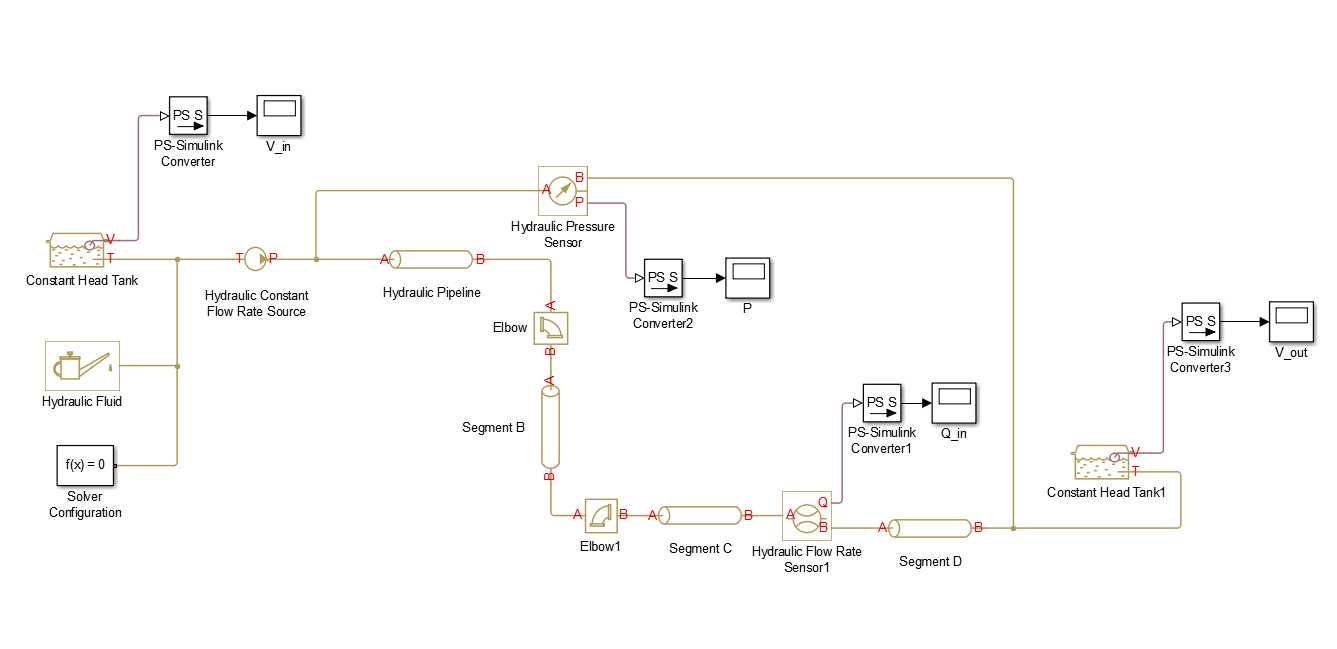
\includegraphics[scale=0.45]{Simulink}
	\caption{Simulink model.}
	\label{fig:simulink}
\end{figure}

A series of simulations with the above model are explored in the following sections.

\section{Part A}
\label{sect:3a}

With the model from Figure~\ref{fig:simulink}, a 20 second simulation is completed for a pipe with inside diameter of 1.50 [in]. Pressure loss, tank volume and flow rates are plotted for flow rate values of 1, 5 and 15 [gpm] (see Figure~\ref{fig:plot150}). Note that all plots were prepared with the \cite{matlab} script found in the Appendix.

\begin{figure}[H]
	\centering
	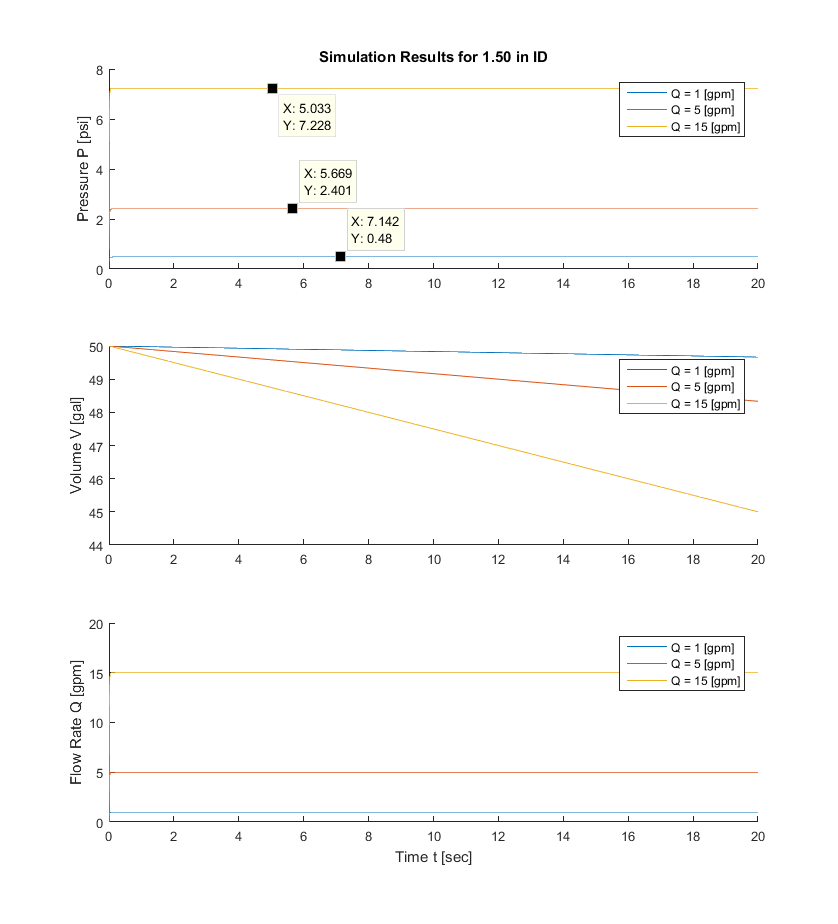
\includegraphics[scale=0.7]{plot150}
	\caption{Pressure loss, tank volume and flow rate plots for $D=1.50$ in.}
	\label{fig:plot150}
\end{figure}

It is clear that as the flow rate increases, the overall pressure drop $\Delta p= p_1 - p_2$ increases from 0.480 to 7.228 [psi]. Furthermore, a decrease in final tank volume is observed with an increase in flow rate $Q$, as expected.

\section{Part B}
\label{sect:3b}

The simulation outlined in Section \ref{sect:3a} is repeated for a pipe with inside diameter of 0.75 [in]. A plotted summary of simulation results is seen below in Figure~\ref{fig:plot075} \cite{matlab}.

\begin{figure}[H]
	\centering
	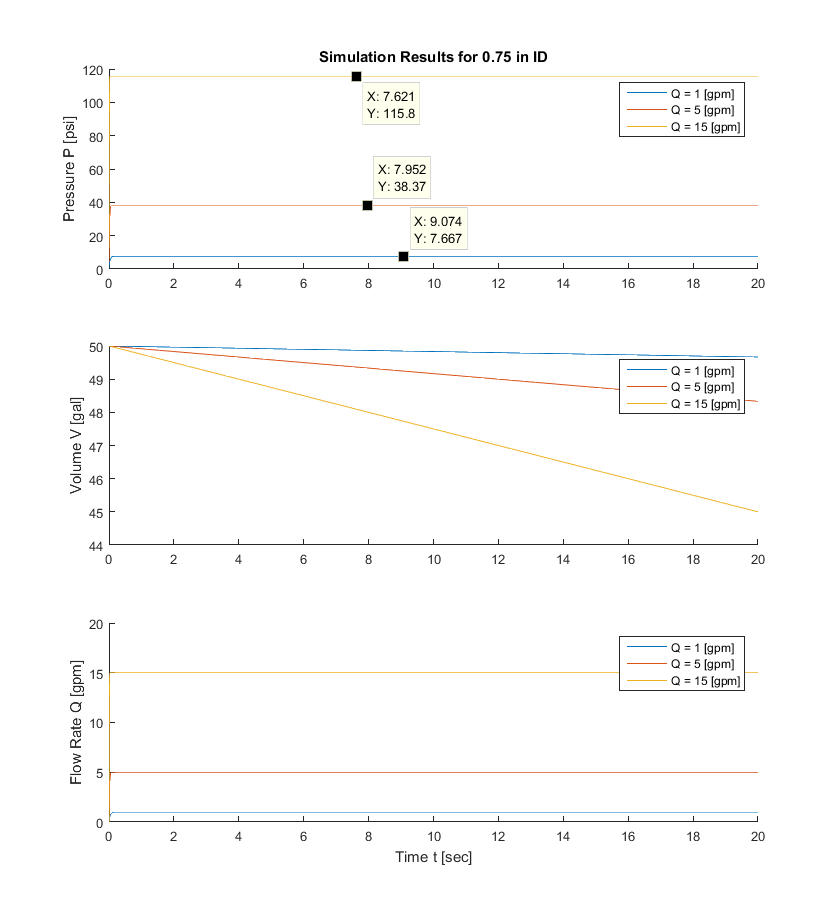
\includegraphics[scale=0.7]{plot075}
	\caption{Pressure loss, tank volume and flow rate plots for $D=0.75$ in.}
	\label{fig:plot075}
\end{figure}

\pagebreak

When comparing the pressure drops experienced by the 1.50 and 0.75 [in] pipes, it can be concluded that there is a large increase in $\Delta p$ with a decrease of inside diameter. Note that tank volume plots remain constant due to the fixed displacement pump.